\chapter{Getting Started with R}


  % location of 
    % not sure this does anything unless we use pgfSweave
         % keep.source probably disables this
          % use pdf for graphics
  % remove blank lines at beginning and end 
  % keeps formatting from original; allows ? to work


\begin{quote}
\emph{This is a lightly modified version of a handout RJP used with his 
Intro Stats students Spring 2011.}
\end{quote}

\label{app:StartingR}

\section{Welcome to \R\ and \Rstudio}

\R\ is a system for statistical computation and graphics.  We will use \R\ in this course 
for several reasons:
\begin{enumerate}
\item \R\ is open-source and freely available for Mac, PC, and Linux machines.
\item \R\ is user-extensible and user extensions can easily be made available to others.
\item \R\ is commercial quality.  It is the package of choice for many statisticians and those
who use statistics frequently.  
\item \R\ is becoming very popular with biologists, especially in certain
sub-disciplines, like genetics.  Articles in research journals such as \textit{Science} often
include links to the \R\ code used for the analysis and graphics presented.
\item
\R\ is very powerful.  Furthermore, it is gaining new features every day.  New statistical 
methods are often available first in \R.
\end{enumerate}

\Rstudio\ provides access to \R\ in a web browser.  The URL is
\begin{center}
\url{http://beta.rstudio.org/}
\end{center}
You shouldbe able to log in using your Calvin ID (\texttt{myname@calvin.edu})  
and KnightVision password.  Once you have logged in, you will see something like 
Figure~\ref{fig:Rstudio-bigview}.

\begin{figure}
\begin{center}
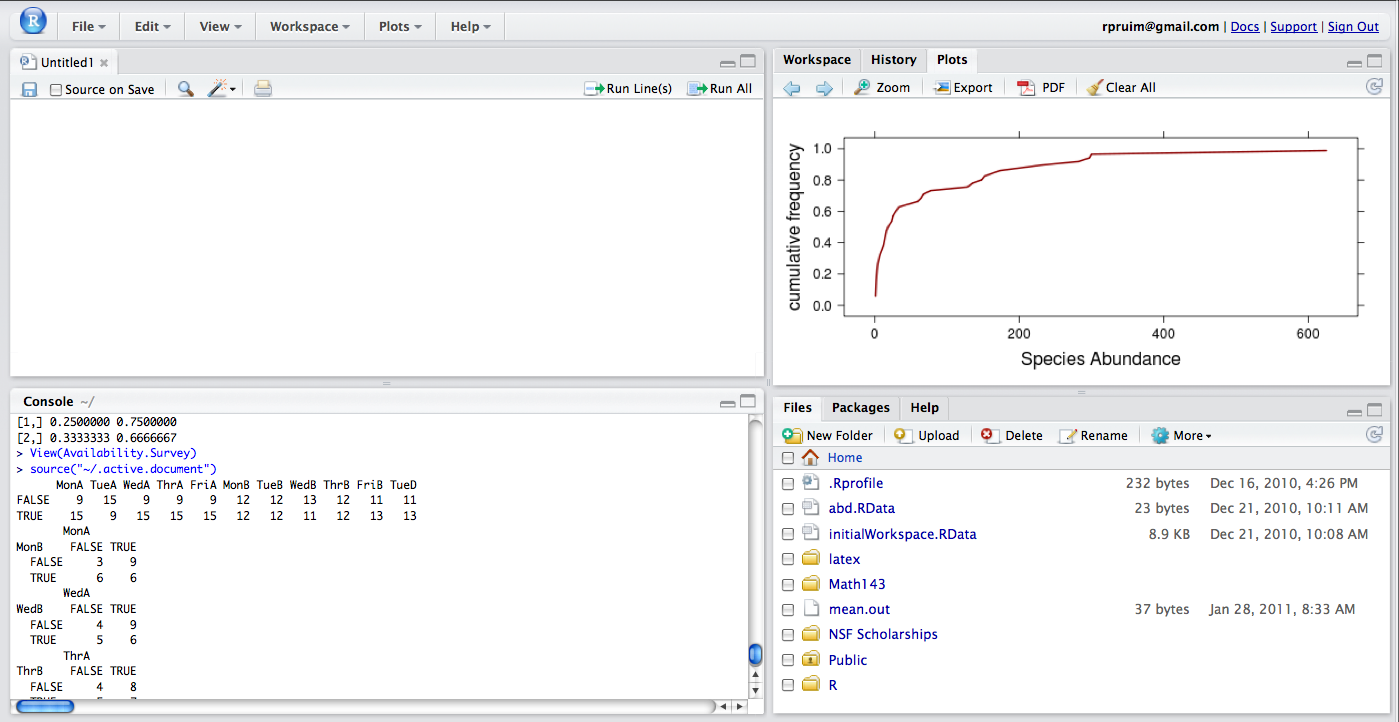
\includegraphics[width=.75\textwidth]{images/RStudio-bigview}
\end{center}
\caption{Welcome to \Rstudio.}
\label{fig:Rstudio-bigview}%
\end{figure}

Notice that \Rstudio\ divides its world into four panels.  Several of the panels
are further subdivided into multiple tabs.
The console panel is where we type commands that \R\ will execute. 

\begin{problem}
Calculate the natural logarithm (log base $e$) and base 10 logarithm of 12,345.
Copy-and-paste your \R\ code into your Word document.  
Be sure to use a fixed-width font (like Courier) when you display \R\ code.  This will
(1) make it clear that you are displaying \R\ input or output, and (2) keep things aligned 
properly.
\end{problem}

\pagebreak
\section{Using R as a Calculator}
\R\ can be used as a calculator.  Try typing the following commands in the console panel.

\begin{Schunk}
\begin{Sinput}
> 5 + 3
\end{Sinput}
\begin{Soutput}
[1] 8
\end{Soutput}
\begin{Sinput}
> 15.3 * 23.4
\end{Sinput}
\begin{Soutput}
[1] 358.02
\end{Soutput}
\begin{Sinput}
> sqrt(16)
\end{Sinput}
\begin{Soutput}
[1] 4
\end{Soutput}
\end{Schunk}
You can save values to named variables for later reuse

\begin{Schunk}
\begin{Sinput}
> product = 15.3 * 23.4       # save result
> product                     # show the result
\end{Sinput}
\begin{Soutput}
[1] 358.02
\end{Soutput}
\begin{Sinput}
> product <- 15.3 * 23.4      # <- is assignment operator, same as =
> product                     
\end{Sinput}
\begin{Soutput}
[1] 358.02
\end{Soutput}
\begin{Sinput}
> 15.3 * 23.4 -> newproduct   # -> assigns to the right
> newproduct
\end{Sinput}
\begin{Soutput}
[1] 358.02
\end{Soutput}
\begin{Sinput}
> .5 * product                # half of the product
\end{Sinput}
\begin{Soutput}
[1] 179.01
\end{Soutput}
\begin{Sinput}
> log(product)                # (natural) log of the product
\end{Sinput}
\begin{Soutput}
[1] 5.880589
\end{Soutput}
\begin{Sinput}
> log10(product)              # base 10 log of the product
\end{Sinput}
\begin{Soutput}
[1] 2.553907
\end{Soutput}
\begin{Sinput}
> log(product,base=2)         # base 2 log of the product
\end{Sinput}
\begin{Soutput}
[1] 8.483896
\end{Soutput}
\end{Schunk}

The semi-colon can be used to place multiple commands on one line.  
One frequent use of this is to save and print a value all in one go:

\begin{Schunk}
\begin{Sinput}
> 15.3 * 23.4 -> product; product    # save result and show it
\end{Sinput}
\begin{Soutput}
[1] 358.02
\end{Soutput}
\end{Schunk}


\subsection*{Four Things to Know About \R}
\begin{enumerate}
\Rwidth=6.25in
\item \R\ is case-sensitive

If you mis-capitalize something in \R\ it won't do what you want.

\item 
Functions in \R\ use the following syntax:

\begin{Schunk}
\begin{Sinput}
> functionname( argument1, argument2, ... )
\end{Sinput}
\end{Schunk}
\vspace{-5mm}
\begin{itemize}
\item The arguments are \underline{always} \emph{surrounded by (round) parentheses} and 
\emph{separated by commas}.

Some functions (like \verb!data()!) 
have no required arguments, but you still need the parentheses.

\item
If you type a function name without the parentheses, you will see the \emph{code} for that
function -- which probably isn't what you want at this point.
\end{itemize}
\item
TAB completion and arrows can improve typing speed and accuracy.

If you begin a command and hit the TAB key, \R\ will show you a list of possible ways to 
complete the command.  If you hit TAB after the opening parenthesis of a function, it will show you
the list of arguments it expects.  The up and down arrows can be used to retrieve past commands.
\item
If you see a \verb!+! prompt, it means \R\ is waiting for more input.

Often this means that you have forgotten a closing parenthesis or made some other
syntax error.  If you have messed up and just want to get back to the normal plot,
hit the escape key and start the command fresh.
\end{enumerate}

\section{R packages}

In addition to its core features, \R\ provides many more features through a (large) number 
of packages.  To use a package, it must be installed (one time), and loaded (each session).
A number of packages are already available in \Rstudio.  
The \tab{Packages} tab in \Rstudio\ will show you the list of installed packages and indicate
which of these are loaded.

\begin{center}
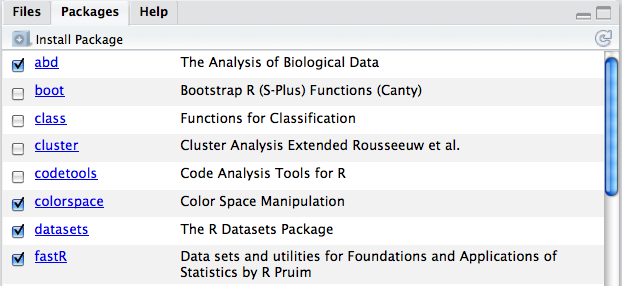
\includegraphics[width=.55\textwidth]{images/RStudio-packages}
\end{center}

%(A similar thing is true for the stand-alone versions of \R.)

Here are some packages we will use frequently in this course:
\begin{itemize}
\item \verb!lattice!  (for graphics; this will always be installed in \R)
\item \verb!Hmisc!    (a package with some nice utilities; available on CRAN)
\item \verb!vcd!      (a package for visualizing categorical data; available on CRAN)
\item \verb!fastR!    (a package with some nice utilities; available on CRAN)
\item \verb!abd!      (a package with data and utilities for our textbook; available on CRAN)
\end{itemize}
There may be others that we use from time to time as well.  You should install
\verb!Hmisc!, \verb!vcd!, \verb!fastR!, \verb!abd!, and \verb!mosaic! 
(in that order) the first time you use \R\ 
so that they are always available to you.
You can install these packages 
by clicking on the ``Install Package" button and following the directions
or by using the following commands:

\begin{Schunk}
\begin{Sinput}
> install.packages('Hmisc')           # note the quotation marks 
> install.packages('vcd')
> install.packages('fastR')
> install.packages('abd')
> install.packages('mosaic')
\end{Sinput}
\end{Schunk}

Once these are installed, you can load them by checking the box in the 
\tab{Packages} tab or by using the commands

\begin{Schunk}
\begin{Sinput}
> require(lattice)
> require(Hmisc)
> require(vcd)
> require(fastR)
> require(abd)
> require(mosaic)
\end{Sinput}
\end{Schunk}

\begin{problem}
Install and load the following packages:
\verb!Hmisc!,
\verb!vcd!,
\verb!fastR!, and 
\verb!abd!.
Make sure \verb!lattice! is also loaded (no need to install it, it is already installed).
\end{problem}


\section{Data}
\subsection{Data in Packages}
Many packages contain data sets.  You can see a list of all data sets in all loaded packages
using 

\begin{Schunk}
\begin{Sinput}
> data()
\end{Sinput}
\end{Schunk}

The \verb!abd! package contains data sets from our text,
\textit{The Analysis of Biological Data}.  The \verb!findData()! function
can help you determine the correct name for the data set you are looking
for.

\begin{Schunk}
\begin{Sinput}
> findData('human')         # all data sets with 'human' in the name
\end{Sinput}
\begin{Soutput}
               name chapter    type number sub
24 HumanGeneLengths       4 Example      1    
43    HumanBodyTemp      11 Example      3    
\end{Soutput}
\end{Schunk}

\begin{Schunk}
\begin{Sinput}
> findData(2)               # all data sets in chapter 2
\end{Sinput}
\begin{Soutput}
                   name chapter    type number sub
1            TeenDeaths       2 Example      1   a
2           DesertBirds       2 Example      1   b
3        SockeyeFemales       2 Example      1   c
4       GreatTitMalaria       2 Example      3    
5            Hemoglobin       2 Example      4    
6               Guppies       2 Example      5   a
7                  Lynx       2 Example      5   b
8     EndangeredSpecies       2 Problem      6    
9       ShuttleDisaster       2 Problem     10    
10          Convictions       2 Problem     16    
11 ConvictionsAndIncome       2 Problem     17    
12            Fireflies       2 Problem     18    
13     NeotropicalTrees       2 Problem     23    
\end{Soutput}
\end{Schunk}

Typically you can use data sets by simply typing their names.  But if you have already
used that name for something or need to refresh the data after making some changes you no longer
want, you can explicitly load the data using the \verb!data()! function with the name of the 
data set you want.

\begin{Schunk}
\begin{Sinput}
> data(iris)
\end{Sinput}
\end{Schunk}

\subsection{Data Frames}

Data sets are usually stored in a special structure called a \term{data frame}.

\begin{boxedText}
Data frames have a 2-dimensional structure.  
\medskip
\begin{itemize}
\item 
Rows correspond to 
\term{observational units} (people, animals, plants, or other objects we
are collecting data about).
\item
Columns correspond to \term{variables} (measurements collected on each 
observational unit).
\end{itemize}
\end{boxedText}

We'll talk later about how to get your own data into \R.  For now we'll use 
some data that comes with \R\ and is all ready for you to use.
The \verb!iris! data frame contains 5 \term{variables} measured for each
of 150 iris plants (the observational units).  
The \verb!iris! data set is included with the default \R\ installation.  
(Technically, it is located in a package called \verb!datasets!  which is always available.)

There are several ways we can get some idea about what is in the \verb!iris! data frame.

\begin{Schunk}
\begin{Sinput}
> str(iris)
\end{Sinput}
\begin{Soutput}
'data.frame':	150 obs. of  5 variables:
 $ Sepal.Length: num  5.1 4.9 4.7 4.6 5 5.4 4.6 5 4.4 4.9 ...
 $ Sepal.Width : num  3.5 3 3.2 3.1 3.6 3.9 3.4 3.4 2.9 3.1 ...
 $ Petal.Length: num  1.4 1.4 1.3 1.5 1.4 1.7 1.4 1.5 1.4 1.5 ...
 $ Petal.Width : num  0.2 0.2 0.2 0.2 0.2 0.4 0.3 0.2 0.2 0.1 ...
 $ Species     : Factor w/ 3 levels "setosa","versicolor",..: 1 1 1 1 1 1 1 1 1 1 ...
\end{Soutput}
\end{Schunk}

\begin{Schunk}
\begin{Sinput}
> summary(iris)
\end{Sinput}
\begin{Soutput}
  Sepal.Length    Sepal.Width     Petal.Length    Petal.Width          Species  
 Min.   :4.300   Min.   :2.000   Min.   :1.000   Min.   :0.100   setosa    :50  
 1st Qu.:5.100   1st Qu.:2.800   1st Qu.:1.600   1st Qu.:0.300   versicolor:50  
 Median :5.800   Median :3.000   Median :4.350   Median :1.300   virginica :50  
 Mean   :5.843   Mean   :3.057   Mean   :3.758   Mean   :1.199                  
 3rd Qu.:6.400   3rd Qu.:3.300   3rd Qu.:5.100   3rd Qu.:1.800                  
 Max.   :7.900   Max.   :4.400   Max.   :6.900   Max.   :2.500                  
\end{Soutput}
\end{Schunk}

\begin{Schunk}
\begin{Sinput}
> head(iris)
\end{Sinput}
\begin{Soutput}
  Sepal.Length Sepal.Width Petal.Length Petal.Width Species
1          5.1         3.5          1.4         0.2  setosa
2          4.9         3.0          1.4         0.2  setosa
3          4.7         3.2          1.3         0.2  setosa
4          4.6         3.1          1.5         0.2  setosa
5          5.0         3.6          1.4         0.2  setosa
6          5.4         3.9          1.7         0.4  setosa
\end{Soutput}
\end{Schunk}
In interactive mode, you can also try

\begin{Schunk}
\begin{Sinput}
> View(iris)
\end{Sinput}
\end{Schunk}
to see the data or 

\begin{Schunk}
\begin{Sinput}
> ?iris
\end{Sinput}
\end{Schunk}
to get the documentation about for the data set.

%\subsection{Getting at the Variables}
Access to an individual variable in a data frame uses the \verb!$! operator in
the following syntax:

\begin{Schunk}
\begin{Sinput}
> dataframe$variable
\end{Sinput}
\end{Schunk}

For example,

\begin{Schunk}
\begin{Sinput}
> iris$Sepal.Length
\end{Sinput}
\begin{Soutput}
  [1] 5.1 4.9 4.7 4.6 5.0 5.4 4.6 5.0 4.4 4.9 5.4 4.8 4.8 4.3 5.8 5.7 5.4 5.1 5.7 5.1 5.4 5.1 4.6
 [24] 5.1 4.8 5.0 5.0 5.2 5.2 4.7 4.8 5.4 5.2 5.5 4.9 5.0 5.5 4.9 4.4 5.1 5.0 4.5 4.4 5.0 5.1 4.8
 [47] 5.1 4.6 5.3 5.0 7.0 6.4 6.9 5.5 6.5 5.7 6.3 4.9 6.6 5.2 5.0 5.9 6.0 6.1 5.6 6.7 5.6 5.8 6.2
 [70] 5.6 5.9 6.1 6.3 6.1 6.4 6.6 6.8 6.7 6.0 5.7 5.5 5.5 5.8 6.0 5.4 6.0 6.7 6.3 5.6 5.5 5.5 6.1
 [93] 5.8 5.0 5.6 5.7 5.7 6.2 5.1 5.7 6.3 5.8 7.1 6.3 6.5 7.6 4.9 7.3 6.7 7.2 6.5 6.4 6.8 5.7 5.8
[116] 6.4 6.5 7.7 7.7 6.0 6.9 5.6 7.7 6.3 6.7 7.2 6.2 6.1 6.4 7.2 7.4 7.9 6.4 6.3 6.1 7.7 6.3 6.4
[139] 6.0 6.9 6.7 6.9 5.8 6.8 6.7 6.7 6.3 6.5 6.2 5.9
\end{Soutput}
\end{Schunk}
shows the contents of the \verb!Sepal.Length! variable.  But this isn't very useful 
for a large data set.  We would prefer to compute numerical or graphical summaries.
We'll do that shortly.

\subsection{Using Your Own Data}
\Rstudio\ will help you import you own data.  To do so use the ``Import Dataset" 
button in the \tab{Workspace} tab.  You can load data from text files, from the web, or from
google spreadsheets.   

%\subsubsection*{From Google Spreadsheets}

\textbf{From Google.}
The easiest of these is the Google spreadsheets option: Just click, select
your spreadsheet, choose a name, and you're done.

%\subsubsection*{From Excel}
\textbf{From Excel},
you need to follow a 3-step process:
\begin{enumerate}
\item
Save your Excel worksheet as a csv file.
\item
Upload (in the \tab{Files} tab) your csv file to the server, where you can create folders and store
files in your personal account.  
(To share things with others: Put the files in your Public folder.  
Read the\texttt{AboutPublic.txt} file in that folder for directions.)
\item
Now import ``from a text file'' in the \tab{Workspace} tab.
\end{enumerate}

In either case, be sure to do the following:
\begin{itemize}
\item Choose good variables names.
\item Put your variables names in the first row.
\item Use each subsequent row for one observational unit.
\item Give the resulting data frame a good name.
\end{itemize}
\authNote{I moved Danny's Simple Relational Database suggestion
to \ref{sec:manipulatingData}.
I don't think I would use a grade/courses example for students nor that
I would introduce \verb!merge()! \emph{et al} to newbies right away.
My goal was to have this appendix look like something that I would give
to students as is in the first week.
In any case, I agree that we should have a section on this somewhere.
[RJP]
}%

\begin{problem}
Enter the following small data set in an Excel or Google spreadsheet and import the 
data into \Rstudio.

\begin{center}
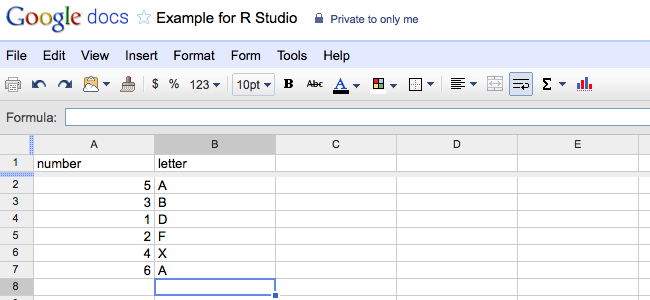
\includegraphics[width=.5\textwidth]{images/GoogleSpreadsheet}
\end{center}

You can import directly from Google.  From Excel, save the file as a csv and
import that (as a text file) into \Rstudio.  Name the data frame \texttt{JunkData}.
Copy and paste the results of 

\begin{Schunk}
\begin{Sinput}
> JunkData
\end{Sinput}
\end{Schunk}
into your report.  (Remember to use a fixed width font like Courier for all \R\ input and 
output.)
\end{problem}


\section{Summarizing Data}

\subsection{A Few Numerical Summaries}
\R\ includes functions that compute a wide range of numerical and graphical summaries.  
Most of the numerical summaries already familiar to you have obvious names.  
Here are a few examples.  (If you don't know what some of these -- like IQR -- are, don't worry;
we'll be discussing them soon.)

\begin{Schunk}
\begin{Sinput}
> mean(iris$Sepal.Length)
\end{Sinput}
\begin{Soutput}
[1] 5.843333
\end{Soutput}
\begin{Sinput}
> median(iris$Sepal.Length)
\end{Sinput}
\begin{Soutput}
[1] 5.8
\end{Soutput}
\begin{Sinput}
> sd(iris$Sepal.Length)
\end{Sinput}
\begin{Soutput}
[1] 0.8280661
\end{Soutput}
\begin{Sinput}
> quantile(iris$Sepal.Length)
\end{Sinput}
\begin{Soutput}
  0%  25%  50%  75% 100% 
 4.3  5.1  5.8  6.4  7.9 
\end{Soutput}
\end{Schunk}

The \verb!favstats()! function in the \verb!abd! package computes several numerical 
summaries all at once.

\begin{Schunk}
\begin{Sinput}
> require(abd)             # if you haven't already loaded the abd package
> favstats(iris$Sepal.Length)
\end{Sinput}
\begin{Soutput}
   median       IQR      mean        sd       var 
5.8000000 1.3000000 5.8433333 0.8280661 0.6856935 
\end{Soutput}
\end{Schunk}

Here's something a little fancier.

\begin{Schunk}
\begin{Sinput}
> summary(Sepal.Length ~ Species, data=iris, fun=favstats)
\end{Sinput}
\begin{Soutput}
Sepal.Length    N=150

+-------+----------+---+------+-----+--------+---------+---------+
|       |          |N  |median|IQR  |mean    |sd       |var      |
+-------+----------+---+------+-----+--------+---------+---------+
|Species|setosa    | 50|5.0   |0.400|5.006000|0.3524897|0.1242490|
|       |versicolor| 50|5.9   |0.700|5.936000|0.5161711|0.2664327|
|       |virginica | 50|6.5   |0.675|6.588000|0.6358796|0.4043429|
+-------+----------+---+------+-----+--------+---------+---------+
|Overall|          |150|5.8   |1.300|5.843333|0.8280661|0.6856935|
+-------+----------+---+------+-----+--------+---------+---------+
\end{Soutput}
\end{Schunk}
(Note: This requires installation of two add-on packages: \verb!Hmsic! 
and \verb!abd!.)

\begin{problem}
What is the average (mean) \emph{width} of the sepals in the \verb!iris! data set?
\end{problem}

\begin{problem}
Determine the average (mean) sepal width for each of the three species in the \verb!iris! data set.
\end{problem}

\subsection{Lattice Graphics}

There are several ways to make graphs in \R.  I like to use a system called
\verb!lattice! graphics.  The first step for using \verb!lattice! is to
load the \verb!lattice! package using the check box in the \tab{Packages} tab or using
the following command:

\begin{Schunk}
\begin{Sinput}
> require(lattice)
\end{Sinput}
\end{Schunk}
\verb!lattice! plots make use of a \term{formula interface}:

\begin{Schunk}
\begin{Sinput}
> plotname( y ~ x | z, data=dataname, groups=grouping_variable, ...)
\end{Sinput}
\end{Schunk}
\begin{itemize}
\item
Our most common plots have the following names:
\begin{itemize}
\item \verb!dotPlot! (notice the capital P; \verb!dotplot()! does something different)
\item \verb!histogram!
\item \verb!bwplot!
\item \verb!xyplot!
\end{itemize}
\item
\verb!x! is the name of the variable that is plotted along the horizontal 
($x$) axis.
\item
\verb!y! is the name of the variable that is plotted along the vertical ($y$) 
axis.  (For some plots, this slot is empty because \R\ computes these values
from the values of \verb!x!.)
\item
\verb!z! is a conditioning variable used to split the plot into 
multiple subplots called \term{panels}.
\item
\verb!grouping_variable! is used to display different groups differently
(different colors or symbols, for example) within the same panel.
\item
\verb!...! There are many additional arguments to these functions that let you
control just how the plots look.  (But we'll focus on the basics for now.)
\end{itemize}

%\subsection*{Some Examples}

\subsection{Dot plots: \texttt{dotPlot()}}

A dot plot represents each value of a quantitative variable with a dot.  The values
are rounded a bit so that the dots line up neatly, and dots are stacked up into little
towers when the data values cluster near each other.

For a dot plot, the \verb!y! component of the formula is empty since we let \R\
calculate that for us.

\begin{center}
\begin{Schunk}
\begin{Sinput}
> dotPlot(~Sepal.Length, data=iris, n=20)   # n=20 gives us approximately 20 towers
\end{Sinput}
\end{Schunk}
\includegraphics{figures/fig-iris-dotPlot}
\end{center}
We can use a conditional variable to give us separate dot plots for each species.

\begin{Schunk}
\begin{Sinput}
> dotPlot(~Sepal.Length|Species, data=iris, n=20)
\end{Sinput}
\end{Schunk}
\begin{center}
\includegraphics{figures/fig-iris-dotPlot-condB}
\end{center}

\subsection{Histograms: \texttt{histogram()}}

Histograms are a lot like dot plots, but the towers of dots are replaced by a vertical bar.
Again the \verb!y! component of the formula is empty since we let \R\
compute the heights of the bars for us.
\begin{center}
\begin{Schunk}
\begin{Sinput}
> histogram(~Sepal.Length, data=iris, n=20)       # n= 20 gives approx. 20 bars
\end{Sinput}
\end{Schunk}
\includegraphics{figures/fig-iris-histogram}
\end{center}
We can use a conditional variable to give us separate histograms for each species.

\begin{center}
\begin{Schunk}
\begin{Sinput}
> histogram(~Sepal.Length|Species, data=iris, n=20)
\end{Sinput}
\end{Schunk}
\includegraphics{figures/fig-iris-histogram-cond}
\end{center}


In lattice lingo, the three subplots are called panels and the 
labels at the top are called strips.  (Strips can be placed on the left side if you 
prefer.)


\subsection{Boxplots:  \texttt{bwplot()}}

Boxplots are made pretty much the same way as histograms:
\begin{center}
\begin{Schunk}
\begin{Sinput}
> bwplot(~Sepal.Length, data=iris)
\end{Sinput}
\end{Schunk}
\includegraphics{figures/fig-iris-bwplot}
\end{center}

We can use conditioning as we did for histograms:

\begin{center}
\begin{Schunk}
\begin{Sinput}
> bwplot(~Sepal.Length|Species, data=iris)
\end{Sinput}
\end{Schunk}
\includegraphics{figures/fig-iris-bwplot-cond}
\end{center}

\vspace{-8mm}

But there are betters ways to do this.
This is better, but the species names run into each other.
\begin{center}
\begin{Schunk}
\begin{Sinput}
> bwplot(Sepal.Length~Species, data=iris)
\end{Sinput}
\end{Schunk}
\includegraphics{figures/fig-iris-bwplot-2d}
\end{center}

We could fix that run-together text by using abbreviated names or rotating the
labels 45 or 90 degrees.  Instead of those solutions, we can also just reverse the roles
of the horizontal and vertical axes.
\begin{center}
\begin{Schunk}
\begin{Sinput}
> bwplot(Species ~ Sepal.Length, data=iris)
\end{Sinput}
\end{Schunk}
\includegraphics{figures/fig-iris-bwplot-2dh}
\end{center}

\vspace{-12mm}

%\pagebreak

\subsection{Scatterplots: \texttt{xyplot()}}

Scatterplots are made with \verb!xyplot()!.  The formula interface is very natural for this.  
Just remember that the ``$y$ variable'' comes first.  (Its label is also farther left on 
the plot, if that helps you remember.)
\begin{center}
\begin{Schunk}
\begin{Sinput}
> xyplot(Sepal.Length ~ Sepal.Width, data=iris)
\end{Sinput}
\end{Schunk}
\includegraphics{figures/fig-iris-xyplot}
\end{center}

Again, we can use conditioning to make a panel for each species.
\begin{center}
\begin{Schunk}
\begin{Sinput}
> xyplot(Sepal.Length ~ Sepal.Width|Species, data=iris)
\end{Sinput}
\end{Schunk}
\includegraphics{figures/fig-iris-xyplot-cond}
\end{center}


Even better (for this example), we can use the \verb!groups! argument to indicate the different species using
different symbols on the same panel.
\begin{center}
\begin{Schunk}
\begin{Sinput}
> xyplot(Sepal.Length ~ Sepal.Width, groups=Species, data=iris)
\end{Sinput}
\end{Schunk}
\includegraphics{figures/fig-iris-xyplot-groups}
\end{center}

\subsection{Saving Your Plots}

There are several ways to save plots, but the easiest is probably the following:
\begin{enumerate}
\item
In the \tab{Plots} tab, click the ``Export'' button.
\item
Copy the image to the clipboard using right click.
\item
Go to your Word document and paste in the image.
\item
Resize or reposition your image in Word as needed.
\end{enumerate}

\subsection{A Few Bells and Whistles}
There are lots of arguments that control how these plots look.  Here are just a few examples.

\subsubsection{auto.key}
It would be useful to have a legend for the previous plot.   \verb!auto.key=TRUE! 
turns on a simple legend.  (There are ways to have more control, if you need it.)
\begin{center}
\begin{Schunk}
\begin{Sinput}
> xyplot(Sepal.Length ~ Sepal.Width, groups=Species, data=iris, 
+ 	auto.key=TRUE)   
\end{Sinput}
\end{Schunk}
\includegraphics{figures/fig-iris-xyplot-key}
\end{center}

\subsubsection{alpha, cex}
Sometimes it is nice to have elements of a plot be partly transparent.  When such
elements overlap, they get darker, showing us where data are ``piling up."
Setting the \verb!alpha! argument to a value between 0 and 1 controls the degree 
of transparency: 1 is completely opaque, 0 is invisible.
The \verb!cex! argument controls ``character expansion" and can be used to make the 
plotting ``characters" larger or smaller by specifying the scaling ratio.
\begin{center}
\begin{Schunk}
\begin{Sinput}
> xyplot(Sepal.Length ~ Sepal.Width, groups=Species, data=iris, 
+ 	auto.key=list(columns=3),
+ 	alpha=.5,
+ 	cex=1.3)   
\end{Sinput}
\end{Schunk}
\includegraphics{figures/fig-iris-xyplot-alpha}
\end{center}

\vspace{-8mm}
\subsubsection*{main, sub, xlab, ylab}

You can add a title or subtitle, or change the default labels of the axes.
\begin{center}
\begin{Schunk}
\begin{Sinput}
> xyplot(Sepal.Length ~ Sepal.Width, groups=Species, data=iris, 
+ 	main="Some Iris Data",
+ 	sub="(R. A. Fisher analysized this data in 1936)",
+ 	xlab="sepal width (cm)",
+ 	ylab="sepal length (cm)",
+ 	alpha=.5,        
+ 	auto.key=list(columns=3))   
\end{Sinput}
\end{Schunk}
\includegraphics{figures/fig-iris-xyplot-text}
\end{center}

\subsubsection{trellis.par.set()}
Default settings for lattice graphics are set using 
\verb!trellis.par.set()!.
Don't like the default font sizes?  You can change to a 7 point (base) font using

\begin{Schunk}
\begin{Sinput}
> trellis.par.set(fontsize=list(text=7))    # base size for text is 7 point 
\end{Sinput}
\end{Schunk}


Nearly every feature of a lattice plot can be controlled: fonts, colors,
symbols, line thicknesses, colors, etc.
Rather than describe them all here, we'll mention only that groups of these settings 
can be collected into a theme.  \verb!show.settings()! will show you what the theme looks like.

\begin{Schunk}
\begin{Sinput}
> trellis.par.set(theme=col.whitebg())      # a theme in the lattice package
> show.settings()
\end{Sinput}
\end{Schunk}
\includegraphics{figures/fig-themes-whitbg}

\begin{Schunk}
\begin{Sinput}
> trellis.par.set(theme=col.abd())          # a theme in the abd package
> show.settings()
\end{Sinput}
\end{Schunk}
\includegraphics{figures/fig-themes-abd}

\begin{Schunk}
\begin{Sinput}
> trellis.par.set(theme=col.mosaic())        # a theme in the mosaic package
> show.settings()
\end{Sinput}
\end{Schunk}
\includegraphics{figures/fig-themes-mosaic}

\begin{Schunk}
\begin{Sinput}
> trellis.par.set(theme=col.mosaic(bw=TRUE)) # black and white version of previous theme
> show.settings()
\end{Sinput}
\end{Schunk}
\includegraphics{figures/fig-themes-mosaicbw}

\begin{Schunk}
\begin{Sinput}
> trellis.par.set(theme=col.abd())          # back to the abd theme
> trellis.par.set(fontsize=list(text=9))    # and back to a 10 point font
\end{Sinput}
\end{Schunk}

\begin{problem}
The \verb!Jordan8687! data set (in the \verb!fastR! package) contains the number 
of points Michael Jordan scored in each game of the 1986--87 season.  
\begin{enumerate}
\item
Make a histogram of this data.  Add an appropriate title.
\item
How would you describe the shape of the distribution?
\item
In approximately what percentage of his games, did Michael Jordan score less than 20 points?
More than 50?
(You may want to add \verb!breaks=seq(0,70,by=5)! to your command to neaten up
the bins.)
\end{enumerate}
\end{problem}

\begin{problem}
Cuckoos lay their eggs in the nests of other birds.  Is the size of cuckoo eggs different
in different host species nests?  The \verb!cuckoo! data set (in \verb!fastR!)
contains data from a study attempting to answer this question.
\begin{enumerate}
\item
When were these data collected?  (Use \verb!?cuckoo! to get information about the data set.)
\item
What are the units on the length measurements?
\item
Make side-by-side boxplots of the length of the eggs by species.
\item
Calculate the mean length of the eggs for each host species.
\item
What do you think?  Does it look like the size is differs among the different host
species?  Refer to your \R\ output as you answer this question.
(We'll learn formal methods to investigate this later in the semester.)
\end{enumerate}
\vspace{-5mm}
\end{problem}

%\subsection{Bar Charts and Pie Charts}
\subsection{Tabulating Categorical Data}
The \verb!Trematodes! data set contains data from an experiment to see if
fish infected with a certain parasite are more likely to be eaten by birds 
(because they swim closer to the surface of the water).  Highly infected, 
lightly infected, and uninfected fish were placed in an outdoor tank that 
was open to foraging birds.  For each fish, the researchers recorded its
infection status and whether it had been eaten.

\begin{Schunk}
\begin{Sinput}
> require(abd)
> head(Trematodes,3)
\end{Sinput}
\begin{Soutput}
    infection.status eaten
1         uninfected   yes
2         uninfected    no
2.1       uninfected    no
\end{Soutput}
\end{Schunk}

\subsubsection{Making Frequency and Contingency Tables with \texttt{xtabs()}}
Categorical variables are  often summarized in a table.  
\R\ can make a table for a categorical variable using \verb!xtabs()!.

\begin{Schunk}
\begin{Sinput}
> xtabs(~infection.status, Trematodes)
\end{Sinput}
\begin{Soutput}
infection.status
      high      light uninfected 
        46         45         50 
\end{Soutput}
\begin{Sinput}
> xtabs(~eaten,Trematodes)
\end{Sinput}
\begin{Soutput}
eaten
 no yes 
 93  48 
\end{Soutput}
\end{Schunk}

%\subsubsection{Cross-Tabulation with \texttt{xtabs()}}
We can make a \term{cross-table} 
(also called a \term{contingency table} or a \term{two-way table}) 
summarizing this data with \verb!xtabs()!.  This is often a more useful view of 
data with two categorical variables.

\begin{Schunk}
\begin{Sinput}
> xtabs( ~ infection.status + eaten, Trematodes)
\end{Sinput}
\begin{Soutput}
                eaten
infection.status no yes
      high        9  37
      light      35  10
      uninfected 49   1
\end{Soutput}
\end{Schunk}

\subsubsection*{Entering Tables by Hand}

Because categorical data is so easy to summarize in a table, 
often the frequency or contingency tables are given instead.
You can enter these tables manually as follows:


\begin{Schunk}
\begin{Sinput}
> myinfection <- c( high=46, light=46, uninfected=50); myinfection
\end{Sinput}
\begin{Soutput}
      high      light uninfected 
        46         46         50 
\end{Soutput}
\end{Schunk}

\label{R:make-xtabs}%
\begin{Schunk}
\begin{Sinput}
> mycrosstable <- rbind(                        # bind row-wise
+                   high = c(no=9, yes=37),     # note labels
+                   light = c(35,10),           # don't need to relabel columns
+                   uninfected = c(49,1)        # note commas throughout
+ 			)
\end{Sinput}
\end{Schunk}

\begin{Schunk}
\begin{Sinput}
> mycrosstable
\end{Sinput}
\begin{Soutput}
           no yes
high        9  37
light      35  10
uninfected 49   1
\end{Soutput}
\end{Schunk}
Replacing \verb!rbind()! with \verb!cbind()! will allow you to give the data
column-wise instead.

\subsection{Graphing Categorical Data}

%\subsubsection{Bar charts and pie charts}
%We won't use these plots often, in part because summary tables are already a good
%way to understand the data.  
The \verb!lattice! function \verb!barchart! can display these tables as barcharts.
\begin{center}
\begin{Schunk}
\begin{Sinput}
> barchart(xtabs(~infection.status, Trematodes))
\end{Sinput}
\end{Schunk}
\includegraphics{figures/fig-barchart1a}
\begin{Schunk}
\begin{Sinput}
> barchart(xtabs(~infection.status, Trematodes), horizontal=FALSE)  # vertical bars
\end{Sinput}
\end{Schunk}
\includegraphics{figures/fig-barchart2a}
\end{center}

\vspace{-6mm}
If the data are already summarized, we can make our bar charts without using
\verb!xtabs()! (Figure~\ref{fig:TeenDeaths-barchart}).

\begin{Schunk}
\begin{Sinput}
> barchart(cause~deaths,TeenDeaths,horizontal=TRUE)
\end{Sinput}
\end{Schunk}
\begin{figure}
\begin{center}
\includegraphics{figures/fig-TeenDeaths-2}
\end{center}
\vspace{-8mm}
\caption{\texttt{barchart(cause\~{}deaths,TeenDeaths,horizontal=TRUE)}}
\label{fig:TeenDeaths-barchart}%
\end{figure}

\iffalse
Statisticians almost never use pie charts.  They are harder to read than bar charts.
The \verb!lattice! package doesn't even include a function to make pie charts.
But the \verb!pie()! function from the \verb!graphics!  package can make these
plots if you absolutely have to have one:

\begin{Schunk}
\begin{Sinput}
> pie(table(Trematodes$infection.status))
> pie(table(Trematodes$eaten))
\end{Sinput}
\end{Schunk}
\fi
\iffalse
\begin{center}
\includegraphics{figures/fig-pie1}
\includegraphics{figures/fig-pie2}
\end{center}
These are probably the last pie charts you will see in this class.
\fi


%\subsubsection{Mosaic plots}

Just as bar charts and pie charts are used to display the distribution
of one categorical variable,  mosaic plots can do the same for cross tables.
\verb!mosaic()! (from the \verb!vcd! package) is not a \verb!lattice! plot, 
but it does use a similar formula interface.  %(See Figure~\ref{fig:mosaic}.)

\begin{Schunk}
\begin{Sinput}
> require(vcd)                              # load the visualing categorical data package
> mosaic(~ infection.status + eaten, Trematodes)
\end{Sinput}
\begin{Soutput}
                 eaten no yes
infection.status             
high                    9  37
light                  35  10
uninfected             49   1
\end{Soutput}
\end{Schunk}


Alternatively, we can send \verb!mosaic()! the output of \verb!xtabs()!:
\begin{center}
\begin{Schunk}
\begin{Sinput}
> mosaic(xtabs(~ infection.status + eaten, Trematodes))
\end{Sinput}
\begin{Soutput}
                 eaten no yes
infection.status             
high                    9  37
light                  35  10
uninfected             49   1
\end{Soutput}
\end{Schunk}
\end{center}

%\vspace{-12mm}
\begin{figure}[h]
\begin{center}
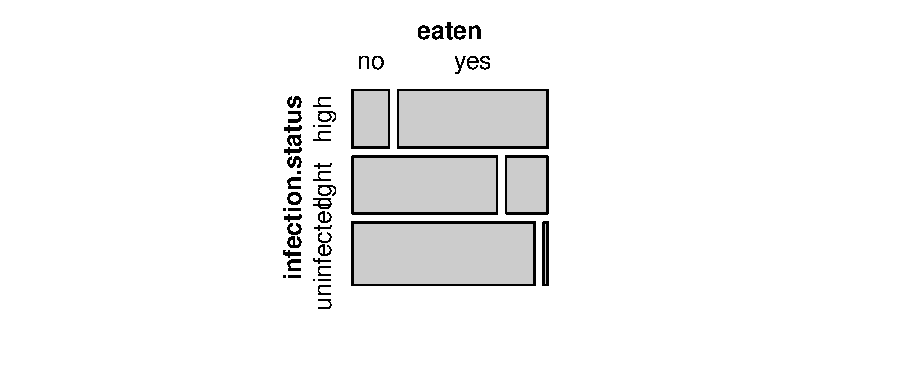
\includegraphics[width=.65\textwidth]{images/fig-mosaic1}
\end{center}
%\caption{\texttt{mosaic(\~{} infection.status + eaten, Trematodes)}}
%\label{fig:mosaic}
\end{figure}

\vspace{-12mm}
Or we can send our own hand-made table (although the output isn't quite as nice without some
extra effort we won't discuss just now):
\begin{center}
\begin{Schunk}
\begin{Sinput}
> mosaic(mycrosstable)
\end{Sinput}
\end{Schunk}
\end{center}

\iffalse
\vspace{-5mm}
Want it the other way around like the other plots?  You can build your table the other way or you can transpose 
the one you have with \verb!t()!:
\begin{center}
\begin{Schunk}
\begin{Sinput}
> mosaic(t(mycrosstable))
\end{Sinput}
\begin{Soutput}
    B high light uninfected
A                          
no       9    35         49
yes     37    10          1
\end{Soutput}
\end{Schunk}
\end{center}
\fi

\iffalse
In these plots, area is proportional to the number in each (combined) category.
This plot makes it easy to see that more infected fish were more likely to be eaten
than less infected fish.
\fi

\begin{problem}
The \verb!utilities2! data set in the \verb!fastR! package contains a number of variables
about the utilities bills at a residence in Minnesota over a number of years.
Since the number of days in a billing cycle varies from month to month, variables 
like \verb!gasbillpday! (\verb!elecbillpday!, etc.) contain the gasbill (electric bill, etc.) 
divided by the number of days in the billing cycle.
\begin{enumerate}
\item
Make a scatter plot of \verb!gasbillpday! vs. \verb!monthsSinceY2K! using the command
\end{enumerate}

\begin{Schunk}
\begin{Sinput}
> xyplot(gasbillpday ~ monthsSinceY2K, data=utilities2, type='l')   # the letter l
\end{Sinput}
\end{Schunk}
\vspace{-6mm}
\begin{enumerate}
\setcounter{enumi}{1}
\item[]
What pattern(s) do you see?
\item
What does \verb!type='l'! do?  Make your plot with and without it.  Which is easier to read
in this situation?
\item
What happens if we replace 
\verb!type='l'! with 
\verb!type='b'!?
\item
Make a scatter plot of \verb!gasbillpday! by \verb!month!.   
What do you notice?

\iffalse
\item
Make side-by-side boxplots of \verb!gasbillpday! by \verb!month!.   
What do you notice?

Your first try probably won't give you what you expect.  The reason is that month is coded
using numbers, so \R\ treats it as numerical data.  We want to treat it as categorical data.
To do this in \R\, use \verb!factor(month)! in place of \verb!month!.  
\R\ calls categorical data a \term{factor}.
\fi
\item
Make any other plot you like using this data.  Include both a copy of your plot and a 
discussion of what you can learn from it.
\end{enumerate}
\end{problem}

\begin{problem}
The table below is from a study of nighttime lighting in infancy and 
eyesight (later in life).  
% latex table generated in R 2.12.1 by xtable 1.5-6 package
% Fri Feb  4 15:46:48 2011
\begin{table}[ht]
\begin{center}
\begin{tabular}{rrrr}
  \hline
 & no myopia & myopia & high myopia \\ 
  \hline
darkness & 155 & 15 & 2 \\ 
  nightlight & 153 & 72 & 7 \\ 
  full light & 34 & 36 & 3 \\ 
   \hline
\end{tabular}
\end{center}
\end{table}

\vspace*{-8mm}

\begin{enumerate}
\item
Do you think this was an experiment or an observational study?  Why?
\item
Recreate the table in \Rstudio.  Copy and paste the results into your Word document.
\item
What percent of the subjects slept with a nightlight as infants?

There are several ways to do this.  You could use \R\ as a calculator to do the arithmetic.
You can save some typing if you use the function \verb!prop.table()!.  See
\verb!?prop.table! for documentation.
If you just want row and column totals added to the table, see \verb!mar_table()!
in the \verb!vcd! package.
\item
Make a mosaic plot for this data.  What does this plot reveal?
\end{enumerate}
\vspace{-5mm}
\end{problem}

%\subsubsection*{More Bar Charts}
\vspace{-8mm}
Barcharts can also be used to display two-way tables.  First we convert
the cross-table to a data frame.
Then we can use this data frame for plotting.

\begin{Schunk}
\begin{Sinput}
> trem <- as.data.frame( xtabs(~ infection.status + eaten, data=Trematodes) ); trem   
\end{Sinput}
\begin{Soutput}
  infection.status eaten Freq
1             high    no    9
2            light    no   35
3       uninfected    no   49
4             high   yes   37
5            light   yes   10
6       uninfected   yes    1
\end{Soutput}
\end{Schunk}

\begin{Schunk}
\begin{Sinput}
> barchart( Freq ~ infection.status, groups=eaten, data=trem) 
\end{Sinput}
\end{Schunk}

\begin{center}
\includegraphics{figures/fig-barchart3}
\end{center}

\vspace{-10mm}
\section{Getting Help}

\subsection{?}

To get help on a specific function or data set, simply precede its name with a \verb!?!:

\begin{Schunk}
\begin{Sinput}
> ?col.whitebg()
\end{Sinput}
\end{Schunk}
%This will give you the documentation for the object you are interested in.

\subsection{\texttt{apropos()}}
If you don't know the exact name of a function, you can give part of the name and 
\R\ will find all functions that match.  Quotation marks are mandatory here.

\begin{Schunk}
\begin{Sinput}
> apropos('hist')            # must include quotes.  single or double.
\end{Sinput}
\begin{Soutput}
 [1] "event.history"              "hist"                       "hist.data.frame"           
 [4] "hist.default"               "hist.FD"                    "hist.scott"                
 [7] "histbackback"               "histochart"                 "histogram"                 
[10] "histogram"                  "history"                    "histSpike"                 
[13] "ldahist"                    "loadhistory"                "panel.histogram"           
[16] "panel.xhistogram"           "panel.xhistogram"           "pmfhistogram"              
[19] "prepanel.default.histogram" "savehistory"                "truehist"                  
[22] "xhistogram"                 "xhistogram"                
\end{Soutput}
\end{Schunk}

\subsection{??}
If that fails, you can do a broader search using \verb!??!, which will find matches not only
in the names of functions and data sets, but also in the documentation for them.
Quotations marks are optional here.

\begin{Schunk}
\begin{Sinput}
> ??histogram                  # any of these will work
> ??"histogram"  
> ??'histogram'  
\end{Sinput}
\end{Schunk}

\subsection{Demos}
The \verb!abd! package also includes demos for some of the sections of the book.
These demos show you how to make the plots or perform the analyses in that section,
so we don't have to repeat them all here.  This also makes it easy to copy and paste
the commands within \Rstudio\ if you need to do something similar.

Here's how \verb!demo()! works.
\begin{center}
\begin{Schunk}
\begin{Sinput}
> demo(sec2.2)
\end{Sinput}
\begin{Soutput}
	demo(sec2.2)
	---- ~~~~~~

> # figure 2.2-1
> cumfreq(~count,DesertBirds, xlab='Species Abundance')
\end{Soutput}
\end{Schunk}
\includegraphics{figures/fig-demo-sec2-2}
\end{center}
\vspace{-8mm}
You can get a list of all available demos using

\begin{Schunk}
\begin{Sinput}
> demo()
\end{Sinput}
\end{Schunk}

\vspace{-8mm}
\section{Additional Notes on R Syntax}


\subsection{Text and Quatations}

For the most part, text in \R\ must be enclosed in either single or double quotations.  
It usually doesn't matter which you use, unless you want one or the other type of 
quotation mark \emph{inside} your text.  Then you should use the other type of 
quotation mark to mark the beginning and the end.

\begin{Schunk}
\begin{Sinput}
> text1 <- "Mary didn't come"            # apostrophe inside requires double quotes around text
> text2 <- 'Do you use "scare quotes"?'  # this time we flip things around
\end{Sinput}
\end{Schunk}

If you omit quotes, you will often see error messages telling you that \R\ can't find 
an object because \R\
will look for a function, data set or other object with that name instead of treating
your text as text.
\begin{Schunk}
\begin{Sinput}
> text3 <- blah
\end{Sinput}
\begin{Soutput}
Error: object 'blah' not found
\end{Soutput}
\end{Schunk}

\subsection{Functions}

Functions in \R\ use the following syntax:

\begin{Schunk}
\begin{Sinput}
> functionname( argument1, argument2, ... )
\end{Sinput}
\end{Schunk}
\vspace{-5mm}
\begin{itemize}
\item The arguments are \underline{always} \emph{surrounded by (round) parentheses} and 
\emph{separated by commas}.
\begin{itemize}
\item
Some functions (like \verb!col.whitebg()!) 
have no arguments, but you still need the parentheses.
\end{itemize}
\item
Most arguments have names, but you don't need to use the names \emph{if you 
give the arguments in the correct order}.  

If you use names, you can give the arguments out of order.  
The following do the same thing,
\end{itemize}

\begin{Schunk}
\begin{Sinput}
> xyplot(Sepal.Length ~ Sepal.Width, data=iris, groups=Species)
> xyplot(Sepal.Length ~ Sepal.Width, iris, groups=Species)
> xyplot(Sepal.Length ~ Sepal.Width, groups=Species, iris)
\end{Sinput}
\end{Schunk}
\begin{itemize}
\item[]
But these do not work
\end{itemize}

\begin{Schunk}
\begin{Sinput}
> xyplot(Sepal.Length ~ Sepal.Width, Species, iris)
> xyplot(Sepal.Length ~ Sepal.Width, iris, Species)
\end{Sinput}
\end{Schunk}
\begin{itemize}
\item[]
The first fails because the second argument is \verb!data!, so \verb!iris!
needs to be in the second position if it is not named.
The second fails because \verb!groups! is not the third argument.
(There are many other arguments between \verb!data! and \verb!groups! .)
The documentation for functions shows the correct order of arguments.
\item
Typically, we will not use names for the first argument or two (these tend to be 
very important arguments that have to be there) but will use names for the rest (these 
are often optional arguments that can be present or not, depending on whether we want 
the default behavior or something special).
\end{itemize}

\section{Installing R}

\subsection{RStudio in the cloud}
Our primary version of \R\ will be the online version of \Rstudio.  
You should have an \Rstudio\ account at \url{http://beta.rstudio.org/} 
using your Calvin student email address and password.
\Rstudio\ is a brand new (and quite nice) interface to \R that runs in a web browser.
This has the advantage that you don't have to install or configure anything.  Just login
and you are good to go.  Futhermore, \Rstudio\ will ``remember'' what you were doing so that
each time you login (even on a different machine) you can pick up right where you left off.
This is ``\R\ in the cloud" and works a bit like GoogleDocs for \R.

If you find bugs or have suggestions for \Rstudio, let me know.  It is in rapid development
at the moment, and I can pass along your feedback to the developers.  You are among the 
first to use \Rstudio, and this is your chance to improve the software!

This should be all you need for this course.  But if you prefer to have a
stand-alone version (because you study somewhere without an internet
connection, for example), read on.


\subsection{RStudio on Your Desktop/Laptop}
There is also a stand-alone version of the \Rstudio\ that you can install on
your desktop or laptop machine.  I'll send you email with instructions indicating where to
find it.  (It is currently in beta and has not been released to the general public.)


\subsection{Getting R from CRAN}

CRAN is the Comprehensive \R\ Archive Network (\url{http://cran.r-project.org/}).  
You can download free versions of \R\ for PC, Mac, and Linux from CRAN.  (If you use
the \Rstudio\ stand-alone version, you also need to install \R\ this way first.)
All the instructions for downloading and installing are on CRAN.  Just 
follow the appropriate instructions for your platform.

\newpage

\section{\R\ Examples}
\vspace{-3mm}
The commands below are illustrated with the data sets \verb!iris! and 
\verb!Trematode!.  To apply these in other situations, you will need to 
substitute the name of your data frame and the variables in it.

\vspace{-3mm}
\begin{center}
\begin{longtable}{p{2.45in}p{4.10in}}
\verb!answer <- 42! & Store the value 42 in a variable named \verb!answer!.
\\[3mm]
%\verb!sl <- iris$Sepal.Length! & Store the \verb!Sepal.Length! variable from the 
%\verb!iris! data frame into a variable called \verb!sl! (to save typing, for example).
%\\[3mm]
\verb!log(123); log10(123); sqrt(123)! & Take natural logarithm, base 10 logarithm, or square 
root of 123.
\\[3mm]
\verb!x <- c(1,2,3)! & Make a variable containing values 1, 2, and 3 (in that order).
\\[3mm]
\verb!data(iris)! & (Re)load the data set \verb!iris!.
\\[3mm]
\verb!findData(2)! & Find \verb!abd! data in chapter 2.
\\[3mm]
\verb!summary(iris$Sepal.Length)! & 
Summarize the distribution of the \verb!Sepal.Length! variable in the \verb!iris! data
frame.
\\[3mm]
\verb!summary(iris)! & 
Summarize each variable in the \verb!iris! data frame.
\\[3mm]
\verb!str(iris)! & A different way to summarize the \verb!iris! data frame.
\\[3mm]
\verb!head(iris)! & First few rows of the data frame \verb!iris!.
\\[3mm]
\verb!require(Hmisc)!

\verb!require(abd)!

\ 
& Load packages.  
(This can also be done by checking boxes in the \tab{Packages} tab.)
\\[3mm]
\multicolumn{2}{l}{
\texttt{summary(Sepal.Length\~{}Species,data=iris,fun=favstats) } 
}
\\[1mm]
& 
Compute favorite statistics of \verb!Sepal.Length! for each \verb!Species!.

[requires \verb!Hmisc! and \verb!abd!]
\\[3mm]
%\verb!cut(x,breaks,right=TRUE)! & Divide up the range of \verb!x! into 
%	intervals and code the values in \verb!x! according to which interval 
%	they fall into. 
%\\[3mm]
\multicolumn{2}{l}{\texttt{histogram(\~{}Sepal.Length|Species,iris)}}
\\[1mm]
& 
Histogram of \verb!Sepal.Length! conditioned on \verb!Species!.
\\[3mm]
\verb!bwplot(Sepal.Length~Species,iris)! & 
Boxplot of \verb!Sepal.Length! conditioned on \verb!Species!.
\\[3mm]
\multicolumn{2}{l}{\texttt{xyplot(Sepal.Length\~{}Sepal.Width|Species,iris)}} 
\\[1mm]
& 
Scatterplot of \verb!Sepal.Length! by \verb!Sepal.Width! 
with separate panels for each  \verb!Species!.
\\[3mm]
\verb!xtabs(~infection.status,Trematodes)! & Frequency table of the variable \verb!infection.status!.
\\[3mm]
\multicolumn{2}{l}{\texttt{barchart(xtabs(\~{}infection.status,Trematodes))}}
\\[1mm]
& Make a barchart from the table.
\\[3mm]
\multicolumn{2}{l}{\texttt{xtabs(\~{}infection.status + eaten,Trematodes)}}
\\[1mm]
& Cross tabulation of \verb!infection.status!  and \verb!eaten!.
\\[3mm]
\multicolumn{2}{l}{
\texttt{mosaic(\~{}infection.status + eaten,Trematodes)} }
\\[1mm]
& Make a mosaic plot.
\\[3mm]
\multicolumn{2}{l}{
\texttt{xtData <- as.data.frame( xtabs(\~{}eaten + infection.status,Trematodes) )}}
\\[1mm]
  & Save cross table information as \verb!xtData!. 
\\[3mm]
\multicolumn{2}{l}{
\texttt{barchart(Freq\~{}infection.status,data=xtData,groups=eaten)}
}
\\[1mm]
& Use \verb!xtData! to make a segmented bar chart.
\\[3mm]
\verb!sum(x)!; 
\verb!mean(x)!; 
\verb!median(x)!;

\verb!var(x)!; 
\verb!sd(x)!; 
\verb!quantile(x)!
& Sum, mean, 
median,
variance,
standard deviation,
quantiles of \verb!x!.
\\
\end{longtable}
%\rule{4in}{1pt}
\end{center}

\vspace*{-.5in}
\section{Exercises}

For these problems, create a single Word document containing all of your work.

\shipoutProblems


